\section{Zielsetzung}
In diesem Experiment wird mithilfe eines Aluminium-Absorbers und eines Streukörpers die sogenannte Compton-Wellenlänge des Elektrons bestimmt, welche eine zentrale konstante im Rahmen des Compton-Effektes ist.
\section{Theorie}
Wenn ein Photon an einem Teilchen, in der Regel wie in diesem Versuch einem Elektron, gestreut wird, kann beobachtet werden, dass sich die Wellenlänge des Photons vergrößert. Diese Verschiebung der Wellenlänge im Rahmen eines Streuprozesses kann beispielsweise bei Röntgen oder $\gamma$-Strahlung beobachtet werden und wird als Compton-Effekt bezeichnet.
Wenn elektromagnetische Strahlung an Materie gestreut wird, wird im allgemeinen zwischen zwei Formen auftretender Streuung, nämlich zum einen der klassischen inelastischen Streuung und zum anderen der elastischen frequenzverschobenen Streuung differenziert. Erstere beschreibt dabei einen Stoßprozess zwischen einem Photon und einem Elektron und wird auch als Compton-Streuung bezeichnet.
\begin{figure} [h]
    \centering
    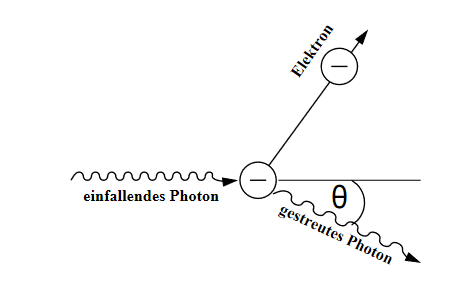
\includegraphics[width=6cm, keepaspectratio]{Compton Effekt}
    \caption{Compton Streuung am Elektron}
    \label{fig:Compton}
 \end{figure}
Bei diesem Prozess wird das Photon am Elektron um den Winkel $\Theta$ von seiner ursprünglichen Bahn abgelenkt und gibt dabei einen Teil seiner Energie an das Elektron ab. Dies führt dazu das sich die Wellenlänge des Photons erhöht. Da sowohl die Energie als auch der Impuls erhalten sind, kann aus den entsprechenden Erhaltungssätzen sowie der Energie-Impuls-Beziehung die Verschiebung der Wellenlänge $\Delta \lambda=\lambda_2-\lambda _1$ als Differenz der Wellenlängen vor ($\lambda_1$) und nach der Streuung ($\lambda_2$) berechnet werden.
\begin{equation}
\Delta \lambda=\frac{h}{m_ec}(1-cos(\Theta))=\lambda_c(1-cos(\Theta))
\end{equation}
Die Konstante $\lambda_c$ wird als Compton-Wellenlänge bezeichnet. Diese Gleichung zeigt, dass die Verschiebung nur
vom Ablenkungswinkel abhängt. Die größtmögliche Verschiebung ergibt sich bei $\Theta=\pi$, während bei einem minnimalen Winkel ($\Theta$=0) keine Streuung und somit keine Verschiebung zustande kommt. \\
Für die Messung der Compton-Wellenlänge wird Rönthgenstrahlung benötigt, welche durch den Beschuss einer Anode mit freien Elektronen zustande kommt. Sie gliedert sich nach der Form ihrer Entstehung in ein charakteristisches Spektrum und ein Bremsspektrum. Ersteres entsteht wenn das Elektron die nötige Energie besitzt, ein Elektron aus einer der unteren Schalen eines Atoms zu lösen. Dies führt dazu, dass ein Elektron aus einer anderen Schale die freie Stelle einnimmt und dabei ein Röntgenquant emmitiert, dessen Energie der Differenz der Bindungenergien der betreffenden Schalen entspricht. Da die Bindungsenergien materialspezifisch sind gilt dies auch für die Linien des characteristischen Spektrums.
Das Bremsspektrum resultiert aus der Ablenkung eines Elektrons im Coulombfeld eines Atomkerns, wobei das Elektron gebremst wird und seine verlorene Energie als Röntgenphoton emmitiert. Da das Elektron beliebig stark abgebremst werden kann ist das daraus resultierende Spektrum kontinuirlich. \\
\begin{figure} [h!]
    \centering
    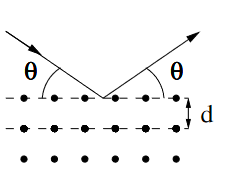
\includegraphics[height=4cm, keepaspectratio]{Bragg-Reflexion}
    \caption{Bragg-Reflexion}
    \label{fig:dings}
 \end{figure}
Um die Wellenlänge der Rönthgenstrahlung zu bestimmen bedient man sich der Bragg-Reflexion. Bei dieser wird die Strahlung gemäß Abbildung $\ref{fig:dings}$ an einem kristallgitter gebeugt. Unter einem bestimmten Winkel $\alpha$ ergibt sich konstruktive Interferenz. Für diesen sogenannten Glanzwinkel kann aus geometrischen Zusammenhängen die Braggsche-Bedingung:
\begin{equation}
2d\sin(\alpha)=n\lambda
\end{equation}
als Zusammenhang zwischen Winkel und Wellenlänge hergeleitet werden. Hier beschreibt $n$ die Ordnung der Beugung und $d$ die Gitterkonstante, welche für einen herkömmlichen LiF-Kristall $214$ pm beträgt. \\
Da zur Messung der Intensität $I$ ein Geiger-Müller-Zählrohr verwendet wird muss auch die sogenannte Totzeit $\tau$ berücksichtigt werden. Diese tritt bei Zählrohren auf und beschreibt den Zeitraum unmittelbar nach registrierung eines Impulses in der kein weiterer Impuls registriert werden kann. Die dadurch nötige Totzeitkorrektur wird mithilfe der Formel:
\begin{equation}
I=\frac{N}{1-\tau N}
\end{equation}  
mit der gemessenen Zählrate $N$ durchgeführt. \\
Zur Bestimmung der Compton-Wellenlänge wird genutzt, dass die Transmission von Rönthgenstrahlung in Materie von der Wellenlänge abhängt. Da die Transmission mit steigender Wellenlänge abnimmt, ist der Transmissionskoeffizient $T$  bei Strahlung, deren Wellenlänge durch den Compton-Effekt erhöht wird, geringer da sie im vergleich zur unverschobenen Strahlung niederenergetischer ist. Die Intensität von Strahlung nimmt in Materie durch Absorption exponentiell mit der Dicke $d$ ab:
\begin{equation}
I=I_0e^{-\mu d}    
\end{equation}
Der Absorptionskoeffizient setzt sich dabei aus drei Komponenten zusammen: $\mu=\mu_{Paar}+\mu_{Photo}+\mu_{Com}$. Diese kommen durch Paarbildung, den Photoeffekt und den Comptoneffekt zustande.
